\section{서론 및 문제 정의}
\label{sec:problem}

PUBG: Battlegrounds와 같은 배틀로얄 장르의 게임에서 한 팀의 최종 순위는 경기
종료 시점에 부여되는 값이지만, 그 순위는 경기 도중 반복되는 생존과 탈락의
순서에 의해 결정된다. 팀은 넓은 맵에 진입해 자원을 확보하고, 다른 팀과의 접촉을
피하거나 감수하며, 점차 축소되는 안전구역 안에서 다음 페이즈를 버텨야 한다.
같은 이동 거리라도 초반의 이동과 후반의 이동은 다른 의미를 갖는다. 초반의 긴
이동은 자원 확보나 위치 선점을 위한 선택일 수 있지만, 후반의 짧은 이동은 블루존
피해, 남은 팀의 밀도, 체력 상태와 결합되어 곧바로 탈락 위험으로 이어질 수 있다.
따라서 PUBG의 순위를 경기 종료 후의 단일 행으로만 다루면, 어떤 팀이 어느
시점에서 위험해졌고 그 위험이 어떤 상태와 이동 이력에서 발생했는지를 잃게 된다.

기존 PUBG 순위 예측 연구는 최종 순위가 데이터로 예측 가능하다는 점을 보여주었다
\cite{kagglePubgFinishPlacement,rokad2019pubgPlacement,sen2021pubgFinalRank,lee2025pubgRank}.
그러나 페이즈별 생존을 묻기 시작하면 문제의 단위가 달라진다. 필요한 것은
``이 팀은 최종적으로 몇 등인가''가 아니라, ``이 팀은 지금까지 관측된 정보만으로
다음 페이즈를 버틸 수 있는가''이다. 이 차이를 다루려면 먼저 로그를 자르는 방식부터
바뀌어야 한다. PUBG 텔레메트리를 경기 후 집계 행이 아니라 이동 객체, 시간변화
영역, 시공간 사건, 페이즈별 위험집합으로 재구성하고, 그 표현이 다음
페이즈의 탈락 위험 예측을 어떻게 가능하게 하는지 확인한다.

본 논문에서 말하는 배틀로얄 장르의 매치는 네 가지 구조를 갖는 게임 플레이
단위로 정의한다. 첫째, 다수의 플레이어 또는 팀이 하나의 경기장 또는 맵에 동시에
배치된다. 둘째, 플레이 가능한 영역은 시간에 따라 축소되고, 그 밖의 영역은
피해를 주는 위험 구역으로 작동한다. 셋째, 팀은 자원, 이동성, 체력, 교전 노출을
관리하며 다음 페이즈까지 생존해야 한다. 넷째, 최종 순위는 각 팀의 탈락 시점에
의해 정해진다. 이 구조를 일반화하면 하나의 매치 \(M\)은 다음과 같이 표현할 수
있다.
\[
M=\langle A,\Omega,T,Z_{1:T},R_{1:T},C_{1:T},S_{1:T},Y\rangle .
\]
여기서 \(A\)는 생존 주체인 플레이어 또는 팀, \(\Omega\)는 경기장 또는 맵,
\(T\)는 매치 시간 또는 페이즈 순서, \(Z_{1:T}\)는 시간에 따라 변하는 안전구역과
위험 구역이다. \(R_{1:T}\)는 아이템, 차량, 회복 수단 같은 자원 상태이고,
\(C_{1:T}\)는 피해, 기절, 처치, 조우 같은 교전 사건이다. \(S_{1:T}\)는 각 주체의
위치와 생존 상태 변화이며, \(Y\)는 탈락 시점과 최종 순위이다. 이 표현에서 순위는
별도의 정적 라벨이 아니라, 페이즈별 위험을 통과하거나 통과하지 못한 순서의 누적
결과다.

그림~\ref{fig:team-phase-st-example}은 이 구조를 실제 PUBG 맵 위에서 보여준다.
한 팀은 낙하지점에서 출발해 페이즈마다 다른 이동 궤적을 남기고, 안전구역 경계가
이동할수록 같은 좌표도 다른 의미를 갖는다. 이 그림에서 중요한 것은 경로의 모양
자체가 아니다. 경로가 어느 페이즈의 어떤 안전구역 안에서, 어떤 탈락 시점으로
이어졌는지가 생존 문제의 단위가 된다.

\begin{figure}[t]
\centering
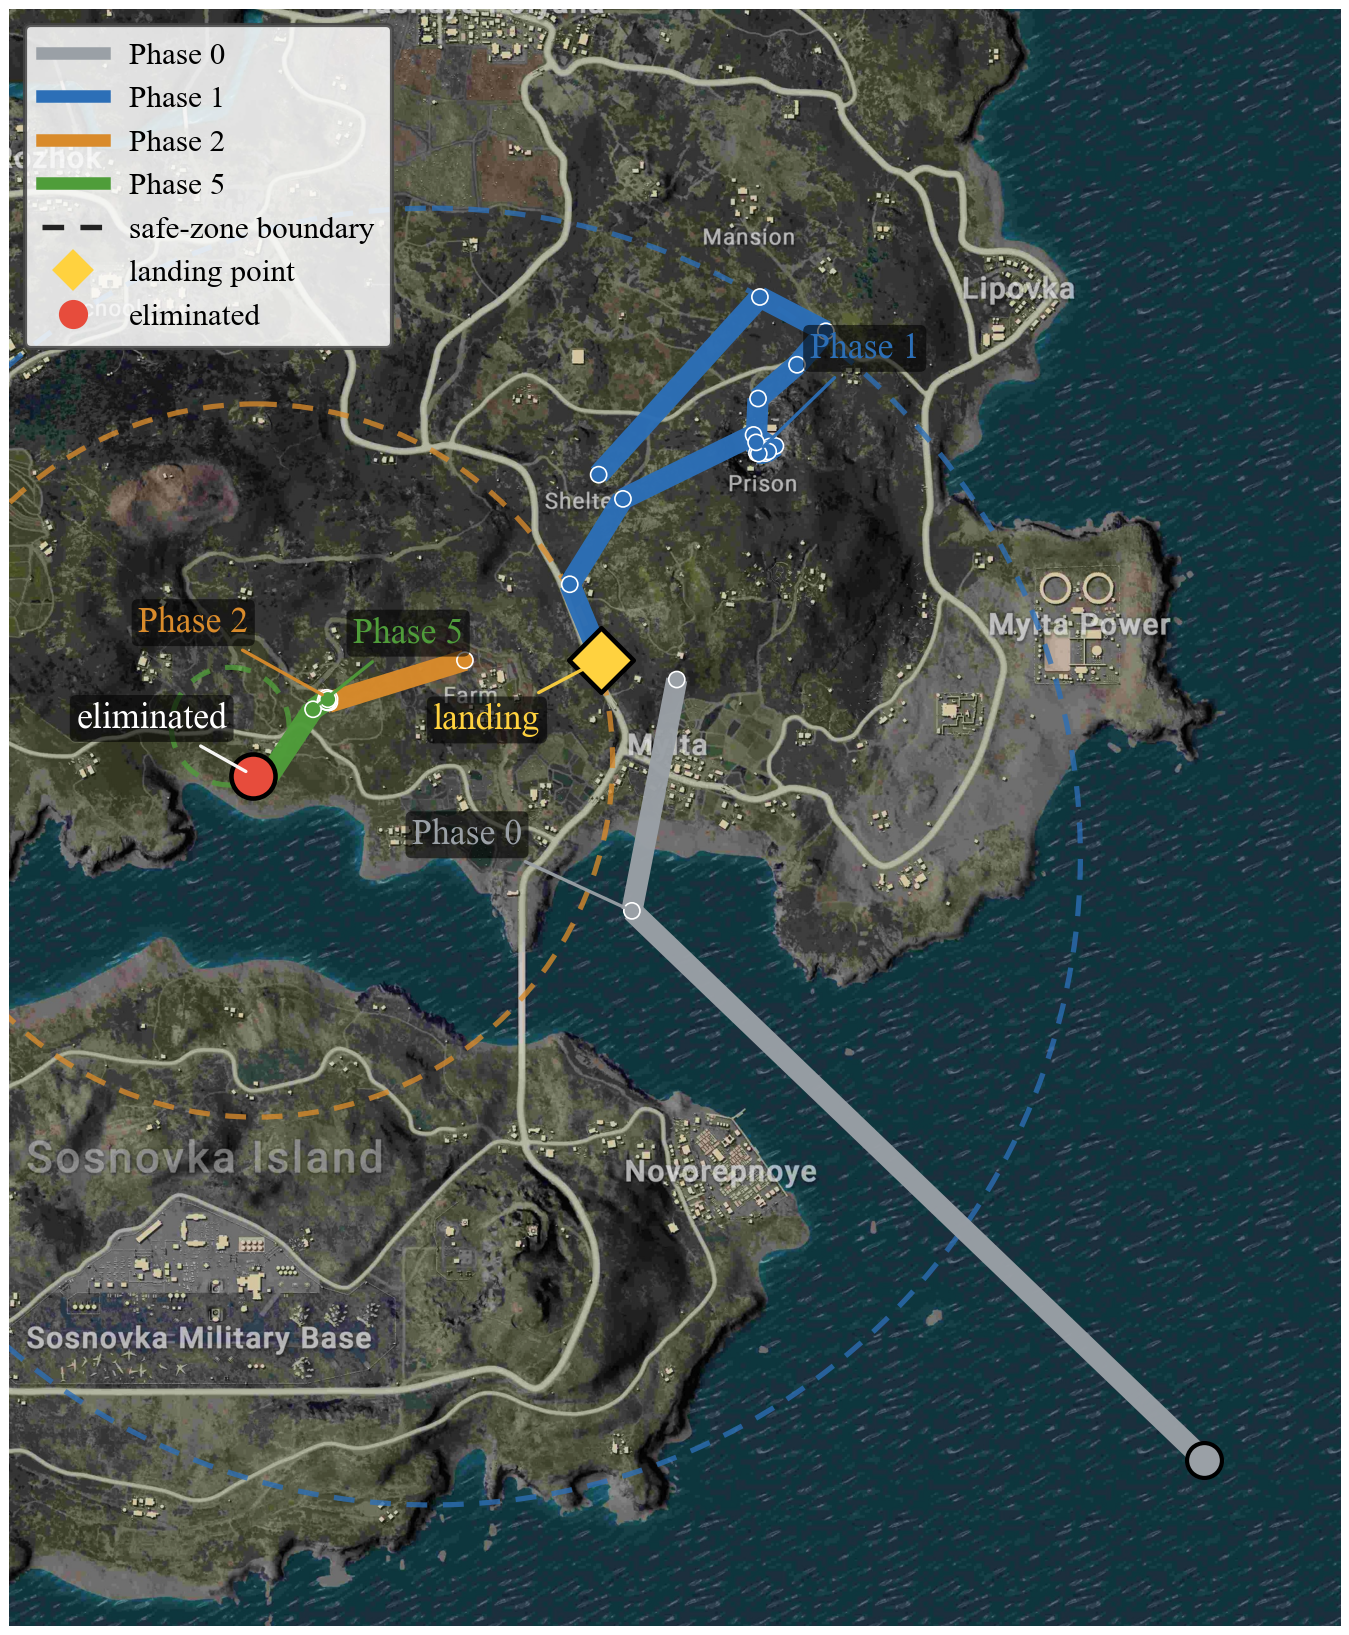
\includegraphics[width=\linewidth]{team_phase_feature_example.png}
\caption{PUBG 텔레메트리를 페이즈별 생존 이력으로 본 예. Erangel 맵 위에 한
팀의 이동 궤적, 페이즈별 안전구역 경계, 낙하지점, 탈락 지점을 함께 표시했다.}
\Description{Erangel 맵 위에 한 팀의 이동 경로와 여러 페이즈의 안전구역 경계,
낙하지점, 탈락 지점을 겹쳐 표시한 시공간 생존 이력 예시.}
\label{fig:team-phase-st-example}
\end{figure}

PUBG: Battlegrounds는 이러한 구조를 관측하기에 적합한 사례이다. 한 매치는 최대
100명의 플레이어를 큰 맵에 배치하고, 안전구역 축소와 블루존 피해 속에서 마지막
생존자를 가린다 \cite{pubgGameInfo}. 공식 개발자 API는 시간순 텔레메트리, 위치
기록, 구역 상태, 교전 사건, 탈락 사건을 제공한다
\cite{pubgDeveloperPortal,pubgTelemetryGuide,pubgTelemetryEvents,pubgTelemetryObjects}.
물론 이 자료가 지형, 엄폐, 시야, 숙련도, 팀 의사소통을 모두 담지는 못한다.
그럼에도 각 팀이 어디에 있었고, 어떤 자원과 체력 상태로 움직였고, 어떤 접촉이나
구역 압력 아래에서 탈락했는지는 재구성할 수 있다.

이 논문의 초점은 특정 예측 모델의 최종 성능 경쟁이 아니다. 먼저 PUBG 텔레메트리를
시공간 데이터베이스 관점에서 어떻게 잘라야 페이즈별 생존 문제가 되는지 묻고, 그
표현이 예측에서 어느 정도 작동하는지 확인한다. 연구 질문은 다음과 같이 좁힌다.

\noindent\textbf{RQ1.} PUBG 스쿼드 매치의 공식 텔레메트리는 이동 객체, 시간변화
영역, 시공간 사건, 페이즈별 위험집합으로 구성된 시공간 데이터베이스
표현으로 재구성될 수 있는가?

\noindent\textbf{RQ2.} 최종 순위 또는 페이즈 종료 시점의 단일 상태로 압축된
표현보다, 페이즈별 시공간 이력을 보존한 표현이 다음 페이즈의 탈락 위험 예측에 더
유용한가?

\noindent\textbf{RQ3.} 직접 생존 상태 변수와 이동 이력, 안전구역 맥락을 분해했을 때
각 구성요소는 다음 페이즈 생존 예측에서 어떤 역할을 하는가?

이 질문들은 특정 모델이나 구성요소가 반드시 우수해야 한다는 가정에서 출발하지
않는다. 중요한 것은 PUBG 스쿼드 매치를 시공간 데이터베이스로 재구성했을 때 생존
예측 문제가 어떻게 정의되고, 어떤 구성요소가 먼저 작동하며, 어떤 구성요소는 더
정교한 표현 설계를 요구하는지 분리하는 것이다.
